\chapter{Digital Repeater Routing Behavior}

When the AX.25 networks were originally built in the 1980s,
one of the fundamental design assumptions was that every node was 
physically static in the network.
Digipeaters were installed on top of high buildings or mountain tops, 
and client nodes were modems connected to bulky video terminals or desktop PCs.
When two stations wanted to exchange packets,
the operators had to manually construct an explicit list of digipeaters to use
to deliver packets to the other station.
Should a station move to a new area, 
the operator would need to discover new near-by digipeaters and manually construct
routing paths using them.

One of the design goals of APRS has been to support mobile nodes,
so this requirement to pre-facto be aware of the
local infrastructure is unacceptable.
The solution was to categorize digipeaters into a small number of ``aliases"
such that a digipeater would respond to both its specific callsign
and to any of its aliases.
A mobile station expecting to move throughout the APRS network
could then construct its routing paths purely out of digipeater aliases
and use the network infrastructure despite not knowing
each digipeater's callsign or location.

As APRS has grown from an experimental network
to one that covers much of the country,
it has adopted and discarded multiple sets of digipeater aliases.
As the expectations as to each node's behavior regarding those aliases have changed,
the APRS community has failed to make it clear that
the previous behavior has been deprecated.
The rest of this chapter will walk through the history
of the basic set of routing aliases,
followed by an overview of possible digipeater behaviors.

More than anything else, this chapter is going to highlight
how ambiguous the APRS specification is in regards to digipeater behavior.
Most of the aliases discussed in the original APRS protocol specification
have been subsequently deprecated,
without the APRS specification being amended to indicate as such.
The APRS specification also failed to have a detailed discussion
on digipeater behavior,
so many different interpretations and ideas have been developed, which has
created several divergent schools of thought on what behavior is best.
Writing a definitive analysis on digipeater behavior is a large undertaking
that warrants further consideration beyond what is possible in this work.

\section{Routing Aliases}

The original definition of APRS included several aliases,
the most notable of which were RELAY and WIDE.
Digipeaters were divided into two categories depending on if they were high-level
(on the top of large towers, mountain tops, etc.)
or low-level (typically residential sites).
Low-level sites would only digipeat packets which used the RELAY alias
or the digipeater's literal callsign,
where high-level digipeaters would respond to both RELAY and WIDE in addition
to their callsign.
This enabled a user to selectively include or exclude the numerous low-level
digipeaters depending on if the station had sufficient power to
reach the high-level WIDE digipeaters or needed the low-level receivers
to assist with being heard on the network.

A station would construct their desired routing path as an ordered list
of callsigns and aliases.
For example, a station requesting three high-level hops out from their position
would use the routing path ``WIDE,WIDE,WIDE" when beaconing in a new area where
the local digipeater callsigns were unknown.
Since these strings of several WIDE aliases proved to be common,
the APRS community developed the concept of WIDEn-N, where multiple
WIDE aliases are summarized as a single routing alias to reduce the average
packet length on the network.

A WIDEn-N alias represents multiple WIDE aliases by using two numbers,
represented by n and N.
The first n represents the originally requested number of WIDE hops,
where the trailing N represents the remaining number of hops that have not yet
been consumed.
Therefore, the alias ``WIDE3-2" represents an original request for three hops
that has already been processed by one digipeater.
Once a WIDEn-N alias gets decremented to WIDEn-0, it is considered entirely
consumed, having been processed by n digipeaters.

Low-level ``fill-in" digipeaters are needed to assist low-power 
moving trackers in reaching the primary high-level digipeater network
before it is possible to be received by other stations.
Without these fill-in digipeaters, 
low power beacons would be lost in the noise and never reach the network at large.
This allows the network to have a very high density of these low-level
digipeaters without all of them generating network traffic by repeating every
packet moving through the network requesting WIDE digipeater service.

\section{Examples}

\begin{figure}
	\centering
	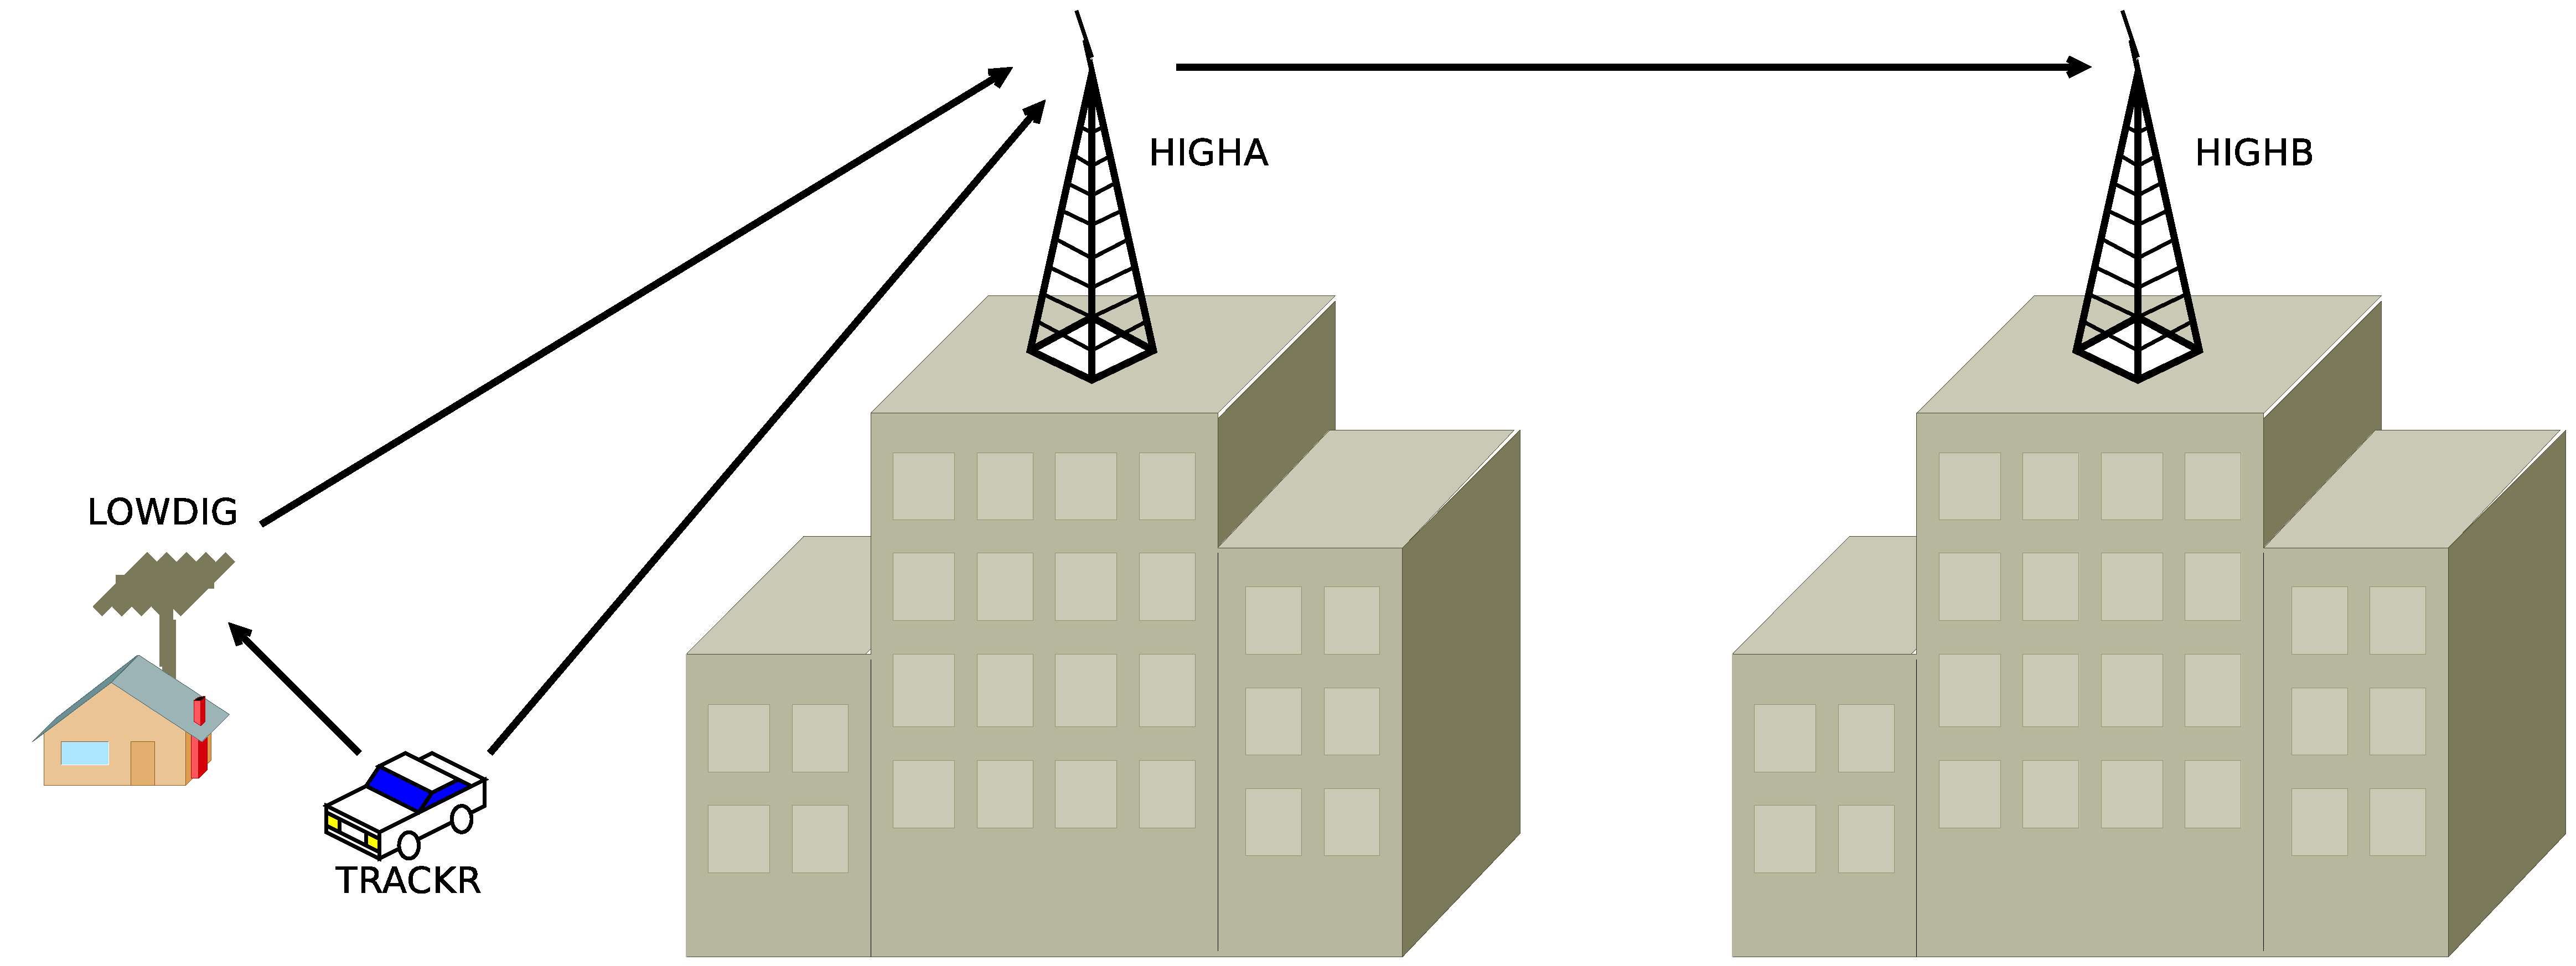
\includegraphics[width=1.0\textwidth]{src/dia/pathdemo}
	\caption{APRS network used for path routing examples}
	\label{fig:pathdemo}
\end{figure}

As an example, consider a small APRS network with one tracker and three
digipeaters as shown in figure \ref{fig:pathdemo}: TRACKR, LOWDIG, HIGHA, and HIGHB.
TRACKR is an APRS tracker originating all of the packets in these examples.
LOWDIG is a low level digipeater that only responds to the RELAY alias, 
where HIGHA and HIGHB are both high-level digis and thus respond to
both RELAY and WIDE.
Consider the routing path sequence in table \ref{tab:singlewide}.
\begin{table}[!h]
	\centering
	\begin{tabular}{ | l | l | }
		\hline
		Path & Transmitted by \\ \hline
		WIDE1-1 & TRACKR \\ \hline
		HIGHA* & HIGHA \\ \hline
		--- & HIGHB \\ \hline
	\end{tabular}
	\caption{TRACKR requesting a single WIDE hop}
	\label{tab:singlewide}
\end{table}

Note the use of the asterisk to represent ``consumed" digipeater hops.
This is originally represented in the binary AX.25 frame
by setting the ``H" bit in the repeater address field.
This notation for the H bit comes from the monitor mode
of the TAPR TNC2, which has become the de-facto standard way to represent
APRS packets textually, such as in log files, documentation, and the
TCP/IP based APRS Internet System backbone.
The TAPR TNC2 also defined the convention to drop the -0 SSID so TRACKR-0 is
written as simply TRACKR.

When HIGHA digipeats this example packet, it appends its callsign to
the list of consumed hops, and should drop the finished "WIDE1*" alias,
which is not consistently implemented in APRS digipeaters.

The ``---" is used in Table \ref{tab:singlewide} to represent that WIDEB does not
repeat this beacon.
It receives the repeated packet from WIDEA, but there are no un-consumed
hops remaining in the path, so the packet is dropped and no one on the other
side of WIDEB would hear this packet.

To reach further out in the network, the user would use a WIDE statement requesting
more than one hop:
\begin{table}[!h]
	\centering
	\begin{tabular}{ | l | l | }
		\hline
		Path & Transmitted by \\ \hline
		WIDE2-2 & TRACKR \\ \hline
		HIGHA*,WIDE2-1 & HIGHA \\ \hline
		HIGHA*,HIGHB* & HIGHB \\ \hline
	\end{tabular}
	\caption{TRACKR requesting two WIDE hops}
	\label{tab:twowide}
\end{table}

If the tracker doesn't happen to reach any of the high-level digis, 
but does reach a low-level one, a WIDE path would do them no good:

\begin{table}[!h]
	\centering
	\begin{tabular}{ | l | l | }
		\hline
		Path & Transmitted by \\ \hline
		WIDE2-2 & TRACKR \\ \hline
		--- & LOWDIG \\ \hline
	\end{tabular}
	\caption{TRACKR requesting WIDE hops but only reaching a relay digi}
	\label{tab:lowhearswide}
\end{table}

Table \ref{tab:lowhearswide} shows that LOWDIG drops the packet since
TRACKR only requests hops from WIDE digipeaters.
Therefore, stations that expect to often be depending on low-level
digipeaters should begin their path with a RELAY alias
as shown in table \ref{tab:lowusingrelay}.

\begin{table}[!h]
	\centering
	\begin{tabular}{ | l | l | }
		\hline
		Path & Transmitted by \\ \hline
		RELAY,WIDE1-1 & TRACKR \\ \hline
		LOWDIG*,WIDE1-1 & LOWDIG \\ \hline
		LOWDIG*,HIGHA* & HIGHA \\ \hline
	\end{tabular}
	\caption{TRACKR using LOWDIG to reach HIGHA}
	\label{tab:lowusingrelay}
\end{table}

Table \ref{tab:usingrelay} is an instance when it's important that high-level
digipeaters also respond to the RELAY alias, since digipeaters traditionally
only process the first unconsumed alias.
Should TRACKR happen to be able to reach HIGHA but be out of range of LOWDIG,
it's desirable for HIGHA to still repeat it.
\begin{table}[!h]
	\centering
	\begin{tabular}{ | l | l | }
		\hline
		Path & Transmitted by \\ \hline
		RELAY,WIDE1-1 & TRACKR \\ \hline
		HIGHA*,WIDE1-1 & HIGHA \\ \hline
		HIGHA*,HIGHB* & HIGHB \\ \hline
	\end{tabular}
	\caption{HIGHA also responding to the RELAY alias}
	\label{tab:usingrelay}
\end{table}

\section{Deduplication Behavior}

As the APRS network grew and the density of digipeaters and stations increased
in the late 1990s and early 2000s,
it became increasingly important that digipeaters don't ``ping-pong" packets
between themselves.
Since APRS' routing is a hop-limited flooding protocol,
there was no mechanism preventing a digipeater from repeating a packet multiple
time.
\begin{table}[!h]
	\centering
	\begin{tabular}{ | l | l | }
		\hline
		Path & Transmitted by \\ \hline
		WIDE3-3 & TRACKR \\ \hline
		HIGHA*,WIDE3-2 & HIGHA \\ \hline
		HIGHA*,HIGHB*,WIDE3-1 & HIGHB \\ \hline
		HIGHA*,HIGHB*,HIGHA* & HIGHA \\ \hline
	\end{tabular}
	\caption{A packet ``ping-ponging" between HIGHA and HIGHB}
	\label{tab:widepingpong}
\end{table}

Table \ref{tab:widepingpong} shows how HIGHA could hear an echo from HIGHB
and transmit the same packet twice, needlessly using additional network bandwidth.
To prevent this, a new behavior was implemented in digipeaters where an
``aging hash table" was used to store a hash of each packet for a limited
length of time (this period is never formally specified, so the author
suggests 30 seconds be used as it is a popular choice).
When a new packet with hops remaining in the path are received,
a hash of the source callsign and Information Field are compared against
the hash table to check if the same packet had been recently transmitted.
If so, the packet is dropped, but if there is no match in the hash table
the packet is digipeated and its hash added to the hash table.
This hash is then dropped from the hash table 30 seconds later to allow
the digipeater to repeat the same packet the next time the original station
beacons it.

\begin{table}[!h]
	\centering
	\begin{tabular}{ | l | l | }
		\hline
		Path & Transmitted by \\ \hline
		WIDE3-3 & TRACKR \\ \hline
		HIGHA*,WIDE3-2 & HIGHA \\ \hline
		HIGHA*,HIGHB*,WIDE3-1 & HIGHB \\ \hline
		--- & HIGHA \\ \hline
	\end{tabular}
	\caption{HIGHA drops the echo heard from HIGHB}
	\label{tab:dropecho}
\end{table}
This behavior, as shown in Table \ref{tab:dropecho},
proved to be tremendously helpful in improving the performance
of the APRS network by removing loops in each packet's flooding behavior.
No quantitative analysis has been found on the subject, but many areas suffering
from congestive collapse reportedly became usable again.

\section{Deprecation of RELAY}

Since APRS was becoming popular among amateur radio operators,
equipment manufacturers such as Kantronics, MFJ, and Kenwood
started adding APRS-specific features into their off-the-shelf TNC products.
One of the most popular TNCs used for digipeater sites was the Kantronics KPC-3+,
which turned out to have a fatal anomaly in its 
version 9.0 firmware ROM regarding the deduplication behavior just
presented \cite{kpc3bugbulletin}.

The KPC-3+ correctly deduplicated packets routed via the WIDEn-N system,
but failed to correctly add to or consult the dedup hash table for single-hop
aliases such as RELAY.
This meant that popular routing paths such as ``RELAY,WIDE2-2" would
still result in routing loops on the network:

\begin{table}[!h]
	\centering
	\begin{tabular}{ | l | l | }
		\hline
		Path & Transmitted by \\ \hline
		RELAY,WIDE2-2 & TRACKR \\ \hline
		RELAY*,WIDE2-2 & HIGHA \\ \hline
		RELAY*,HIGHB*,WIDE2-1 & HIGHB \\ \hline
		RELAY*,HIGHB*,HIGHA* & HIGHA \\ \hline
	\end{tabular}
	\caption{HIGHA failing to dedup its prior RELAY}
	\label{tab:kpc3fail}
\end{table}

Kantronics did release a patched ROM v9.1 in 2007, but to insufficient effect.
Getting access to digipeaters at remote radio sites is burdensome,
and physically replacing the 32 pin ROM chip inside the KPC-3+ 
with a \$40 replacement\footnote{Kantronics did offer free v9.1 ROM exchanges to 
any customers who had purchased their TNCs new in the previous two years} 
proved to be a sufficient barrier that many APRS digipeaters still
suffer from this defect today.\footnote{It has been jokingly said 
	that once a digipeater goes on the air,
	none of its settings will be changed until either the digipeater
or its owner dies}

Due to this growing population of digipeaters suffering from the Kantronics or other
misinterpretations of the RELAY,WIDE alias system, 
it was proposed that APRS switch to a purely WIDEn-N routing method. 
Instead of low-level digipeaters responding to RELAY,
they should now only process the alias WIDE1-1.
This means that a path such as ``RELAY,WIDE2-2" should now be rewritten as
``WIDE1-1,WIDE2-2." 
To digipeaters aware of this new interpretation, ``WIDE1-1,WIDE2-2" signifies 
requesting one low-level and two high-level hops.
To older digipeaters like the KPC-3+, it appears to be an odd way to request
three WIDE hops compared to ``WIDE3-3," 
yet the deduplication is still done correctly.

The issue with this replacement of RELAY with WIDE1-1 is that there is now
no way to correctly request a single high-level hop.
The solution was to allow trackers to use the alias of WIDE2-1 for single
high level hops.
This works, but now breaks the original meaning of the first number,
which stood for the originally requested number of hops.
When a digipeater receives a packet with a ``WIDE2-1" path, 
there is no way to definitively
tell if that alias represents a two hop request that has gone through one hop,
or a single high-level hop request that hasn't been processed yet.

Surprisingly, this single overload of WIDE2-1 for WIDE1-1 has rendered the
original meaning of the first digit almost meaningless.
Allowing this one exception to the originating station setting the two WIDEn-N
numbers the same, while not providing sufficient documentation
to make it abundantly clear that this is the only allowable exception,
has muddied the waters as to the actual meaning of the first number.
Based on a sample of 21 million packets on the APRS-IS world-wide APRS 
backbone on May 8th, 2014, it was found that
0.7\% of APRS packets requested routing paths such as WIDE1-2 or WIDE2-3,
which should not ever exist before or after the WIDE2-1 exception was made..
A station beaconing with a path of WIDE2-3 indicates that they are requesting
two hops, and three of those hops are remaining, which is nonsense.\footnote{The
proper way to request three hops would be to use WIDE3-3.}
This demonstrates that users are clearly confused and that a
major institutional failure has occurred in how the meaning of the WIDEn-N alias has
been presented.

\section{Minimum WIDEn-N Behavior}

APRS digipeaters are divided into two classes: high-level digipeaters and
low-level digipeaters, which dictates variations in their behavior.
High-level digipeaters form the major backbone of the APRS digipeater network
and are generally installed on the tops of mountains,
tall office buildings, and large towers.
Low-level digipeaters usually have their antennas less than 50 feet above ground
level, and cover a small subset of the wider coverage provided by the
nearest high-level digipeater.

Since each low-level digipeater's coverage area is a subset of the
nearest high-level digipeater's coverage, a low-level digi isn't needed
to repeat packets coming in from the high-level digipeater.
Low-level digipeaters are designed to solely act as ``boosters" to
help local low-power trackers be able to reach the nearest high-level digi.
Therefore, low-level digipeaters should only digipeat packets which
have ``WIDE1-1" as their first routing hop, since that indicates that
the user doesn't believe they can reach high-level digipeaters directly.

High-level digipeaters form the actual blanket coverage of APRS, and
should respond to any valid WIDEn-N alias which still contains unconsumed hops,
including WIDE1-1. This is because many digipeaters will only consume the first
unused alias in the path, so a low-power tracker that gets ``lucky" and manages to
reach a high-level digipeater while using a path such as ``WIDE1-1,WIDE2-2"
depends on high-level digipeaters responding to WIDE1-1.

Digipeater behavior includes several more caveats which don't involve the APRS
WIDEn-N routing alias,\footnote{Examples include the expectation of digipeaters
	to substitute their callsigns into routing paths as they consume aliases,
	and that they still must respond to their callsign as a routing hop in 
addition to the WIDEn-N alias.} 
so this section can't be considered a complete definition of a digipeater's behavior.

\section{Variations on Digipeater Behavior}

As previously mentioned, the failure of the APRS specification to provide
a comprehensive extension of digipeater behavior for APRS has caused
implementers to get creative with the details and extensions of
the basic behavior defined in the AX.25 specification.
Some of these variations include:
\begin{itemize}
	\item How should the last hop of multi-hop aliases be handled?\footnote{i.e.
		should ``WIDE3-1" become ``DIGIA*" or ``DIGIA*,WIDE3*"?}
	\item Preemptive digipeating, where digipeaters consider all
		unused aliases, instead of only the first,
		and possibly consumes multiple hop requests if an alias match is
		found later in the path.
	\item Long path traps, where abusive WIDE paths such as WIDE7-7 are trapped
		and all or many requested hops are consumed by the first digipeater,
		to prevent flooding extremely large areas.
	\item Direct-only digipeaters, where low-level digipeaters don't only respond
		to WIDE1-1, but only digipeat packets when they appear to have not
		been already digipeated by another digipeater.
	\item Viscous delay digipeaters, where packets are held for a number of
		seconds to see if they are otherwise re-transmitted by other digipeaters.
		If an echo of a packet is heard, it gets dropped instead of digipeated.
	\item Token bucket digipeaters, which refuse to digipeat stations which
		exceed a specified volume of network traffic.
\end{itemize}

While the implications of any single item on this list are seemingly small,
the countless permutations and inconsistencies seen deployed in the
world-wide APRS network causes the network to behave unpredictably and
give disappointing levels of service to its end-users.
Further work is needed to specify how much of a digipeater's behavior is
required versus optional, and how much latitude should be given to individual
digipeater operators for any of the optional features implemented.

